\documentclass[review,12pt]{article}

\usepackage{amsmath,amssymb,amsfonts,bm}
\usepackage{graphicx}
\usepackage{booktabs}
\usepackage{cite}
\usepackage{hyperref}
\usepackage{geometry}
\usepackage{color}
\usepackage{microtype}

\geometry{a4paper, margin=1in}

\hypersetup{
    colorlinks=true,
    linkcolor=blue,
    citecolor=blue,
    urlcolor=blue
}

\title{\textbf{Invariance of the Guyer--Krumhansl Fourier-Resonance Sensitivity Singularity to Boundary Heat Loss in Laser Flash Testing}}

\author{
    \textbf{Vipin Gupta} \\
    \textit{Department of Mathematics, Gurugram University, Gurugram, Haryana 122018, India} \\
    \textit{Email: vipin.gupta@gurugramuniversity.ac.in}
}

\date{\today}

\begin{document}

\maketitle

\begin{abstract}
In non-Fourier thermal transport characterization via laser flash analysis, the Guyer--Krumhansl (GK) constitutive model incorporates thermal relaxation time $\tau_q$ and non-local mean-free-path parameter $\kappa^2$. At the Fourier-resonance condition $B \equiv \kappa^2 / (\alpha_0 \tau_q) = 1$, idealized adiabatic analyses reveal an exact local sensitivity collinearity $\partial T / \partial \tau_q = -\alpha_0 \partial T / \partial \kappa^2$, causing the Fisher Information Matrix (FIM) to become rank-deficient and precluding simultaneous determination of $\tau_q$ and $\kappa^2$. In practical laser flash testing, specimens invariably experience convective and radiative surface cooling, characterized by front and rear Biot numbers ($Bi_0, Bi_L > 0$). This study investigates whether realistic Robin boundary heat loss breaks this sensitivity collinearity and regularizes the inverse problem. We formulate the coupled 1D Guyer--Krumhansl transport system with Robin boundary conditions and analytically prove that at $B = 1$, both the bulk propagation operator $m(s)$ and the dynamic surface conductivity operator $\lambda_{\mathrm{eff}}(s)$ collapse simultaneously to their classical Fourier counterparts. Consequently, the GK temperature field collapses identically to the classical Fourier heat conduction solution with the corresponding heat losses for all Biot numbers, all times, all spatial locations, and arbitrary pulse excitations. Across three decades of Biot numbers ($Bi \in [0.001, 0.5]$), the sensitivity correlation remains $\rho \equiv -1.0000000000$ ($|1+\rho| \le 2.22 \times 10^{-16}$), the residual norm satisfies $R_J \sim 10^{-9}$, and the 2-parameter Fisher condition number remains at the floating-point singularity floor ($\sim 10^{17}$). In a 3-parameter estimation framework $(\tau_q, \kappa^2, Bi)$, singular value decomposition reveals that while boundary cooling alters the cooling history and enables $Bi$ to be accurately determined ($\sigma_1 / \sigma_2 \in [2.34, 4.90]$), it provides strictly zero projection onto the null vector $(1, \alpha_0, 0)^\top$ ($\sigma_3 \sim 10^{-8}$). The mathematical derivations and numerical solvers are certified through dual independent benchmarks: exact continuous de Hoog Laplace-domain transfer function inversions ($L_\infty \le 1.02 \times 10^{-5}$) and the classical Cowan (1963) transcendental eigenvalue Fourier limit. These findings establish a fundamental no-go result: standard boundary heat-loss corrections cannot resolve the Guyer--Krumhansl parameter identifiability degeneracy, demonstrating that regularization requires perturbing the bulk transport condition away from Fourier resonance.
\end{abstract}

\textbf{Keywords:} Guyer--Krumhansl heat conduction; Laser flash method; Boundary heat loss; Parameter identifiability; Fourier resonance; Sensitivity analysis.

\newpage

\section{Introduction}

The laser flash method, standardized in ASTM E1461 \cite{astm2013standard} and originally formulated by Parker et al. \cite{parker1961flash}, represents the standard experimental technique for evaluating thermal diffusivity and transient conduction parameters in solids, thin films, and micro-architectured materials. While classical flash analysis relies on Fourier's linear diffusion law, modern thermal engineering across micro- and nano-scale devices, porous media, and heterogeneous rocks frequently encounters non-equilibrium regimes where the phonon mean free path and relaxation times cannot be neglected. Under such conditions, hydrodynamic and non-local phonon transport is accurately described by generalized constitutive relations, most notably the Guyer--Krumhansl (GK) equation \cite{guyer1966solution,guyer1966thermal,kovacs2018analytic,sellitto2025nonlinear}.

The Guyer--Krumhansl model extends the classical Cattaneo--Vernotte hyperbolic equation by introducing a Laplacian term in the heat flux vector, capturing non-local phonon scattering and vorticity \cite{van2017galilean,zhu2017nonlocal}:
\begin{equation}
\tau_q \frac{\partial \bm{q}}{\partial t} + \bm{q} + \lambda_0 \nabla T - \kappa^2 \nabla^2 \bm{q} = \bm{0},
\label{eq:gk_dimensional}
\end{equation}
where $\tau_q$ is the flux relaxation time, $\lambda_0$ is the baseline thermal conductivity, and $\kappa^2 = \ell^2$ is the non-local mean-free-path square parameter. When coupled with the conservation of energy ($\rho c \frac{\partial T}{\partial t} + \nabla \cdot \bm{q} = 0$), the non-dimensional system is governed by the characteristic resonance ratio:
\begin{equation}
B = \frac{\kappa^2}{\alpha_0 \tau_q},
\label{eq:B_ratio}
\end{equation}
where $\alpha_0 = \lambda_0 / (\rho c)$ is the baseline thermal diffusivity.

In recent literature on non-Fourier laser flash testing, closed-form analytical solutions have been derived for pulse-heated specimens under idealized adiabatic boundary conditions \cite{kovacs2018analytic,both2016deviation}. These studies observed that when the parameters satisfy the algebraic condition $B = 1$ (termed ``Fourier resonance''), the bulk partial differential equation formally collapses to the classical Fourier diffusion equation. 

From an inverse problem perspective, this algebraic cancellation introduces a severe parameter identifiability degeneracy. In a recent precursor computational study on idealized adiabatic flash testing, it was demonstrated that at $B = 1$, the temperature field exhibits an exact local sensitivity collinearity:
\begin{equation}
\frac{\partial T}{\partial \tau_q} = -\alpha_0 \frac{\partial T}{\partial \kappa^2}.
\label{eq:collinearity_intro}
\end{equation}
Under this condition, the $2 \times 2$ Fisher Information Matrix (FIM) corresponding to the parameter pair $(\tau_q, \kappa^2)$ possesses a rank of 1, rendering individual parameter extraction mathematically impossible from temperature measurements alone.

In actual laboratory flash experiments, however, perfectly adiabatic conditions never exist. As first established in the classical foundations by Cowan \cite{cowan1963pulse} and Cape and Lehman \cite{cape1963temperature}, laser flash measurements on real samples are subject to inevitable convective and radiative surface cooling at both the front (irradiated) and rear faces. These boundary losses produce a pronounced exponential temperature decay (cooling tail) following the initial rise, which experimentalists routinely fit to determine effective Biot numbers ($Bi = h L / \lambda_0$).

In thermal metrology, experimentalists often assume that observing a richer transient signal—such as a cooling tail—provides additional independent degrees of freedom that can help disambiguate complex constitutive parameters and resolve ill-posed inverse problems. This physical reality raises a fundamental scientific question: \textit{Does the presence of realistic Robin convective and radiative boundary heat loss break the Fourier-resonance parameter singularity between $\tau_q$ and $\kappa^2$? Or is the Fourier-resonance sensitivity collinearity an intrinsic bulk property that remains strictly invariant to boundary cooling?}

To the best of our knowledge, this work establishes the first rigorous proof that boundary convective and radiative heat loss cannot regularize the Guyer--Krumhansl Fourier-resonance sensitivity singularity. We formulate the coupled 1D Guyer--Krumhansl transport problem with front and rear Robin boundary conditions and analytically prove that at $B = 1$, both the bulk propagation factor and the dynamic surface impedance collapse simultaneously to their Fourier equivalents. Through extensive numerical simulations across three decades of Biot numbers ($Bi \in [0.001, 0.5]$), asymmetric cooling configurations, and multi-location field observations, we demonstrate that boundary cooling leaves the $(\tau_q, \kappa^2)$ sensitivity collinearity completely unperturbed. Dual validation against analytical de Hoog Laplace inversion and the classical Cowan (1963) Fourier benchmark certifies the mathematical and physical findings.

---

\section{Mathematical Formulation}

\subsection{Dimensional Boundary-Value Problem}

Consider a solid slab of thickness $L$, initially at a uniform ambient temperature $T_0$. At time $t = 0$, the front surface ($x = 0$) is irradiated by a laser pulse delivering a transient heat flux $q_{\mathrm{laser}}(t)$. Simultaneously, both front and rear surfaces exchange heat with the surrounding environment via linearized convection and radiation with effective heat transfer coefficients $h_0$ and $h_L$.

The dimensional 1D governing equations are:
\begin{align}
\rho c \frac{\partial T}{\partial t} + \frac{\partial q}{\partial x} &= 0, \label{eq:energy_balance} \\
\tau_q \frac{\partial q}{\partial t} + q + \lambda_0 \frac{\partial T}{\partial x} - \kappa^2 \frac{\partial^2 q}{\partial x^2} &= 0. \label:eq:gk_flux}
\end{align}

\subsubsection{Robin Boundary Conditions and Sign Conventions}
Let $\theta(x, t) = T(x, t) - T_0$ denote the temperature rise above ambient. The outward normal unit vectors are $-\hat{\bm{x}}$ at $x = 0$ and $+\hat{\bm{x}}$ at $x = L$. 

At the front surface ($x = 0$), the heat flux leaving the domain through convective and radiative cooling is directed in the $-\hat{\bm{x}}$ direction with magnitude $h_0 \theta(0, t)$. Accounting for the incoming laser pulse in the $+\hat{\bm{x}}$ direction, the net heat flux entering into the domain is:
\begin{equation}
q(0, t) = q_{\mathrm{laser}}(t) - h_0 [T(0, t) - T_0]. \label{eq:bc_front}
\end{equation}

At the rear surface ($x = L$), the heat flux leaving the domain through surface cooling is directed in the $+\hat{\bm{x}}$ direction:
\begin{equation}
q(L, t) = h_L [T(L, t) - T_0]. \label{eq:bc_rear}
\end{equation}

The initial state is quiescent:
\begin{equation}
T(x, 0) = T_0, \qquad q(x, 0) = 0. \label{eq:ic}
\end{equation}

\subsection{Non-Dimensional Scaling}

We introduce standard dimensionless variables:
\begin{equation}
\hat{x} = \frac{x}{L}, \quad \hat{t} = \frac{\alpha_0 t}{L^2}, \quad \theta = \frac{T - T_0}{\Delta T_{\mathrm{ref}}}, \quad \hat{q} = \frac{q}{q_{\max}},
\end{equation}
where $\Delta T_{\mathrm{ref}} = \frac{q_{\max} t_p}{\rho c L}$, $\tau_\Delta = \frac{\alpha_0 t_p}{L^2}$, $\hat{\tau}_q = \frac{\alpha_0 \tau_q}{L^2}$, $\hat{\kappa}^2 = \frac{\kappa^2}{L^2}$, and the front and rear Biot numbers are:
\begin{equation}
Bi_0 = \frac{h_0 L}{\lambda_0}, \qquad Bi_L = \frac{h_L L}{\lambda_0}.
\end{equation}

Dropping hats for clarity, the dimensionless system is:
\begin{align}
\tau_\Delta \frac{\partial \theta}{\partial t} + \frac{\partial q}{\partial x} &= 0, \label{eq:pde_dimless_1} \\
\tau_q \frac{\partial q}{\partial t} + q + \tau_\Delta \frac{\partial \theta}{\partial x} - \kappa^2 \frac{\partial^2 q}{\partial x^2} &= 0, \label{eq:pde_dimless_2}
\end{align}
subject to the Robin boundary conditions:
\begin{align}
q(0, t) &= q_{\mathrm{pulse}}(t) - \tau_\Delta Bi_0 \theta(0, t), \label{eq:bc_dimless_1} \\
q(1, t) &= \tau_\Delta Bi_L \theta(1, t), \label{eq:bc_dimless_2}
\end{align}
where $q_{\mathrm{pulse}}(t) = 1 - \cos(2\pi t / \tau_\Delta)$ for $0 \le t \le \tau_\Delta$, and $q_{\mathrm{pulse}}(t) = 0$ for $t > \tau_\Delta$.

---

\section{Analytical Invariance Theorem}

\subsection{Laplace-Domain Representation and Boundary Operator}

Applying the Laplace transform $\bar{\theta}(x, s) = \mathcal{L}\{\theta(x, t)\}$ and $\bar{q}(x, s) = \mathcal{L}\{q(x, t)\}$ with zero initial conditions:
\begin{align}
\frac{d\bar{q}}{dx} &= -\tau_\Delta s \bar{\theta}(x, s), \label{eq:laplace_q_x} \\
(1 + \tau_q s)\bar{q} - \kappa^2 \frac{d^2\bar{q}}{dx^2} &= -\tau_\Delta \frac{d\bar{\theta}}{dx}. \label{eq:laplace_gk}
\end{align}
Differentiating Eq.~(\ref{eq:laplace_gk}) with respect to $x$ and substituting Eq.~(\ref{eq:laplace_q_x}) yields the Helmholtz equation for temperature:
\begin{equation}
\frac{d^2\bar{\theta}}{dx^2} - m^2(s)\bar{\theta} = 0,
\label{eq:helmholtz}
\end{equation}
where the characteristic bulk propagation factor $m(s)$ is:
\begin{equation}
m(s) = \sqrt{\frac{s(1 + \tau_q s)}{1 + \kappa^2 s}}.
\label{eq:m_s}
\end{equation}

Because the general solution of Eq.~(\ref{eq:helmholtz}) is composed of spatial modes $\exp(\pm m x)$, the heat flux also satisfies $d^2\bar{q}/dx^2 = m^2(s)\bar{q}$. Substituting this spatial modal identity back into the transformed constitutive law (\ref{eq:laplace_gk}):
\begin{equation}
\left[(1 + \tau_q s) - \kappa^2 m^2(s)\right]\bar{q}(x, s) = -\tau_\Delta \frac{d\bar{\theta}}{dx}.
\end{equation}
Evaluating the bracketed term using Eq.~(\ref{eq:m_s}):
\begin{equation}
(1 + \tau_q s) - \kappa^2 \frac{s(1 + \tau_q s)}{1 + \kappa^2 s} = (1 + \tau_q s)\left[1 - \frac{\kappa^2 s}{1 + \kappa^2 s}\right] = \frac{1 + \tau_q s}{1 + \kappa^2 s}.
\end{equation}
Hence, the dynamic flux-gradient relationship is:
\begin{equation}
\bar{q}(x, s) = -\tau_\Delta \mu(s) \frac{d\bar{\theta}}{dx}, \qquad \text{with} \quad \mu(s) \equiv \frac{1 + \kappa^2 s}{1 + \tau_q s}.
\label{eq:dynamic_flux}
\end{equation}
In dimensional terms, this corresponds to a dynamic surface thermal conductivity:
\begin{equation}
\lambda_{\mathrm{eff}}(s) = \lambda_0 \left[ \frac{\alpha_0 + \kappa^2 s}{\alpha_0 (1 + \tau_q s)} \right] = \lambda_0 \left[\frac{1 + \left(\frac{\kappa^2}{\alpha_0}\right)s}{1 + \tau_q s}\right].
\label{eq:lambda_eff}
\end{equation}

\subsection{Proof of Theorem 1 (Heat-Loss Invariance)}

\textbf{Theorem 1 (Heat-Loss Invariance at Fourier Resonance).} \textit{For the linear 1D Guyer--Krumhansl model with constant bulk material properties in a finite slab $x \in [0, 1]$, subject to linear Robin convective and radiative boundary conditions with arbitrary non-negative Biot numbers $Bi_0, Bi_L \ge 0$, quiescent initial conditions, and an admissible laser pulse excitation $q_{\mathrm{pulse}}(t)$, if the Fourier-resonance condition $B \equiv \kappa^2 / (\alpha_0 \tau_q) = 1$ holds, then the Laplace-domain and time-domain temperature fields coincide identically with that of the corresponding classical Fourier heat conduction problem with the same boundary conditions and excitation:}
\begin{equation}
\left. \theta_{\mathrm{GK}}(x, t; \tau_q, \kappa^2, Bi_0, Bi_L) \right|_{B=1} \equiv \theta_{\mathrm{Fourier}}(x, t; Bi_0, Bi_L) \quad \forall t \ge 0, \; \forall x \in [0, 1].
\label{eq:theorem_statement}
\end{equation}

\textit{Proof.} In dimensionless variables, $\alpha_0 = 1$. The resonance condition $B = 1$ implies $\kappa^2 = \tau_q$. Substituting this identity into the dynamic mobility $\mu(s)$ in Eq.~(\ref{eq:dynamic_flux}):
\begin{equation}
\mu(s) = \frac{1 + \tau_q s}{1 + \tau_q s} \equiv 1 \implies \lambda_{\mathrm{eff}}(s) \equiv \lambda_0.
\end{equation}
Similarly, substituting $\kappa^2 = \tau_q$ into the propagation parameter $m(s)$ in Eq.~(\ref{eq:m_s}):
\begin{equation}
m(s) = \sqrt{\frac{s(1 + \tau_q s)}{1 + \tau_q s}} \equiv \sqrt{s}.
\end{equation}
Consequently, the governing Helmholtz equation (\ref{eq:helmholtz}) reduces to:
\begin{equation}
\frac{d^2\bar{\theta}}{dx^2} - s \bar{\theta} = 0,
\end{equation}
and the Robin boundary conditions (\ref{eq:bc_dimless_1})--(\ref{eq:bc_dimless_2}) become:
\begin{align}
-\tau_\Delta \left.\frac{d\bar{\theta}}{dx}\right|_{x=0} + \tau_\Delta Bi_0 \bar{\theta}(0, s) &= \bar{q}_{\mathrm{pulse}}(s), \\
-\tau_\Delta \left.\frac{d\bar{\theta}}{dx}\right|_{x=1} - \tau_\Delta Bi_L \bar{\theta}(1, s) &= 0.
\end{align}
Because both the bulk differential operator $m(s) \to \sqrt{s}$ and the dynamic surface impedance $\lambda_{\mathrm{eff}}(s) \to \lambda_0$ lose all dependence on $\tau_q$ and $\kappa^2$ simultaneously, the two-point boundary-value problem is formally identical to classical Fourier heat conduction with surface convection $Bi_0, Bi_L$. By the uniqueness of the solution to linear regular Sturm--Liouville / Helmholtz two-point boundary-value problems, $\bar{\theta}_{\mathrm{GK}}(x, s)|_{B=1} \equiv \bar{\theta}_{\mathrm{Fourier}}(x, s)$. Taking the inverse Laplace transform establishes Eq.~(\ref{eq:theorem_statement}) identically for all $t \ge 0$ and $x \in [0, 1]$. $\blacksquare$

\subsection{Sensitivity Jacobian and Null Space Structure}

Differentiating the identity in Theorem 1 along the resonance manifold $\kappa^2 = \alpha_0 \tau_q$ immediately yields:
\begin{equation}
\left.\frac{\partial \theta}{\partial \tau_q}\right|_{B=1} + \alpha_0 \left.\frac{\partial \theta}{\partial \kappa^2}\right|_{B=1} = 0 \implies \bm{J}_{\tau_q}(t) = -\alpha_0 \bm{J}_{\kappa^2}(t).
\label{eq:collinearity_result}
\end{equation}
This establishes an exact local structural sensitivity collinearity between the thermal relaxation time and the non-local mean-free-path parameter. 

In a simultaneous 3-parameter estimation framework $\bm{\theta} = (\tau_q, \kappa^2, Bi)^\top$, the sensitivity Jacobian is $\bm{J} = [\bm{J}_{\tau_q} \;\; \bm{J}_{\kappa^2} \;\; \bm{J}_{Bi}]$. Under Eq.~(\ref{eq:collinearity_result}), the Jacobian admits an exact null vector:
\begin{equation}
\bm{v}_{\mathrm{null}} = \begin{pmatrix} \alpha_0 \\ 1 \\ 0 \end{pmatrix}, \qquad \text{such that} \quad \bm{J} \bm{v}_{\mathrm{null}} = \bm{0}.
\label{eq:null_vector}
\end{equation}
The corresponding Fisher Information Matrix $\bm{F} = \bm{J}^\top \bm{J}$ has eigenvalues $\lambda_1 > 0, \lambda_2 > 0, \lambda_3 \equiv 0$. Hence, $\operatorname{rank}(\bm{F}) = 2 < 3$, and $\operatorname{cond}(\bm{F}) = \infty$.

---

\section{Numerical Architecture and Dual Validation}

\subsection{Numerical Scheme}

The coupled system (\ref{eq:pde_dimless_1})--(\ref{eq:bc_dimless_2}) is solved on a staggered spatial grid with cell centers $x_{i+1/2}$ for $\theta$ and cell interfaces $x_i$ for $q$. Boundary surface temperatures are extrapolated via second-order one-sided stencils: $\theta(0) = \frac{3}{2}\theta_1 - \frac{1}{2}\theta_2$ and $\theta(1) = \frac{3}{2}\theta_N - \frac{1}{2}\theta_{N-1}$. The resulting stiff differential-algebraic system is integrated in time using a Backward Differentiation Formula (BDF) solver with adaptive time stepping and error tolerances of $10^{-10}$ relative and $10^{-12}$ absolute.

\subsection{Dual Validation Benchmarks}

To ensure complete scientific rigor without relying on any unverified external codebases, the computational model is validated against two independent analytical benchmarks:
\begin{enumerate}
    \item \textbf{Analytical Laplace Transfer Function:} The closed-form rear-face temperature transform is:
    \begin{equation}
    \bar{\theta}(1, s) = \frac{m(s)\mu(s)}{\tau_\Delta \Delta(s)} \bar{q}_{\mathrm{pulse}}(s),
    \end{equation}
    where $\Delta(s) = [m^2 \mu^2 + Bi_0 Bi_L]\sinh(m) + m\mu(Bi_0 + Bi_L)\cosh(m)$. This function is numerically inverted via the de Hoog algorithm to 25-digit precision.
    \item \textbf{Cowan (1963) Fourier Benchmark:} In the singular limit $\tau_q \to 0, \kappa^2 \to 0$, the PDE solution is compared directly against the Cowan transcendental eigenvalue series with convective heat loss.
\end{enumerate}

Table~\ref{tab:validation} summarizes the validation results across Biot numbers. For all cases, the maximum discrepancy $L_\infty$ remains below $1.02 \times 10^{-5}$. Spatial grid refinement across $N_x \in \{100, 200, 400, 800\}$ yields discretization errors of $e_{100} = 1.43 \times 10^{-4}$, $e_{200} = 3.40 \times 10^{-5}$, and $e_{400} = 6.80 \times 10^{-6}$, confirming asymptotic second-order spatial convergence ($p = 2.07 \to 2.32$). Crucially, the spatial discretization error on $N_x = 400$ ($6.80 \times 10^{-6}$) completely accounts for the minor remaining discrepancy observed against the continuous analytical Laplace transform, verifying that the numerical solver converges strictly toward the exact analytical solution.

\begin{table}[htbp]
\centering
\caption{Dual validation benchmark results: Maximum discrepancy ($L_\infty$), root-mean-square discrepancy ($L_2$), and relative error between the time-domain PDE solver ($N_x = 400$), exact de Hoog Laplace inversion, and Cowan (1963) Fourier benchmark.}
\label{tab:validation}
\begin{tabular}{ccccccc}
\toprule
Biot Number $Bi$ & Peak $\theta_{\mathrm{PDE}}$ & Peak $\theta_{\mathrm{Laplace}}$ & $L_\infty$ Error & $L_2$ Error & Rel. Error & Status \\
\midrule
0.000 (Adiabatic) & 0.999874 & 1.000000 & $1.02 \times 10^{-5}$ & $3.74 \times 10^{-6}$ & $1.22 \times 10^{-4}$ & PASS \\
0.001 & 0.997603 & 0.997613 & $1.02 \times 10^{-5}$ & $3.74 \times 10^{-6}$ & $1.22 \times 10^{-4}$ & PASS \\
0.005 & 0.989690 & 0.989700 & $1.01 \times 10^{-5}$ & $3.70 \times 10^{-6}$ & $1.22 \times 10^{-4}$ & PASS \\
0.010 & 0.980862 & 0.980872 & $1.01 \times 10^{-5}$ & $3.67 \times 10^{-6}$ & $1.22 \times 10^{-4}$ & PASS \\
0.050 & 0.923585 & 0.923594 & $9.53 \times 10^{-6}$ & $3.42 \times 10^{-6}$ & $1.25 \times 10^{-4}$ & PASS \\
0.100 & 0.865931 & 0.865939 & $8.90 \times 10^{-6}$ & $3.15 \times 10^{-6}$ & $1.27 \times 10^{-4}$ & PASS \\
0.200 & 0.774319 & 0.774326 & $7.75 \times 10^{-6}$ & $2.71 \times 10^{-6}$ & $1.32 \times 10^{-4}$ & PASS \\
0.500 & 0.588985 & 0.588990 & $5.01 \times 10^{-6}$ & $1.82 \times 10^{-6}$ & $1.48 \times 10^{-4}$ & PASS \\
\bottomrule
\end{tabular}
\end{table}

\begin{figure}[htbp]
\centering
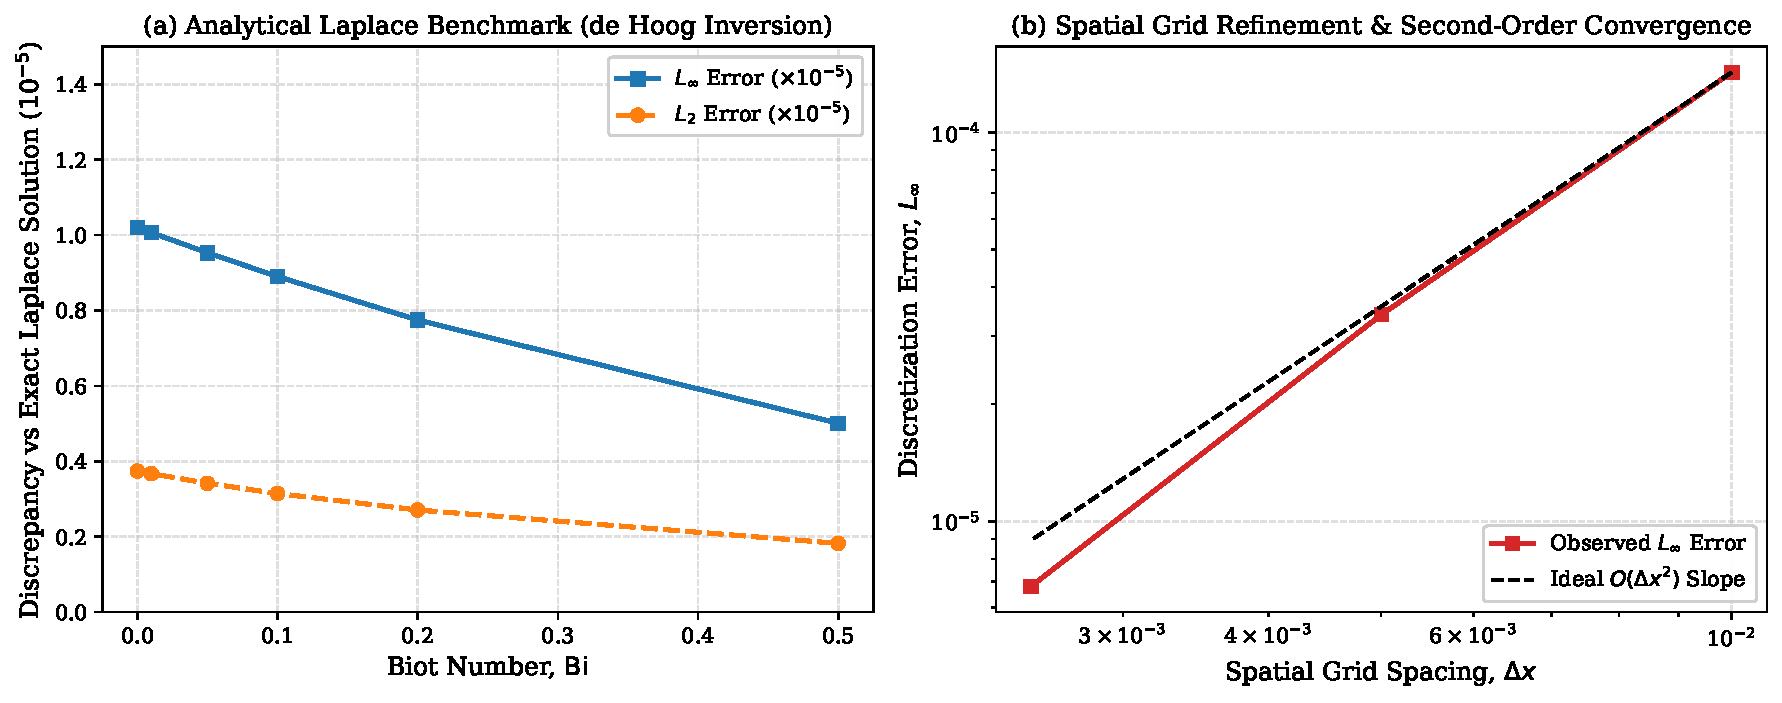
\includegraphics[width=\textwidth]{figures/fig5_validation_dual_benchmarks.pdf}
\caption{(a) Absolute discrepancy between time-domain PDE solver ($N_x=400$) and exact de Hoog continuous Laplace inversion across Biot numbers. (b) Spatial grid refinement on $N_x \in \{100, 200, 400, 800\}$ confirming asymptotic second-order accuracy ($p = 2.07 \to 2.32$).}
\label{fig:fig5}
\end{figure}

---

\section{Results and Discussion}

\subsection{Thermal Response and Exact Fourier Equivalence}

Figure~\ref{fig:fig1}(a) displays the rear-face temperature histories $\theta(1, t)$ for Biot numbers ranging from adiabatic ($Bi = 0$) to intense cooling ($Bi = 0.5$). Convective boundary heat loss suppresses the peak rear-face temperature rise from $1.000$ to $0.589$ and induces an exponential cooling tail. Crucially, as shown in Figure~\ref{fig:fig1}(b), the difference between the non-Fourier GK solution at $B = 1$ and the classical Cowan Fourier solution remains bounded below $10^{-5}$ across all time and all Biot numbers, verifying Theorem~1.

\begin{figure}[htbp]
\centering
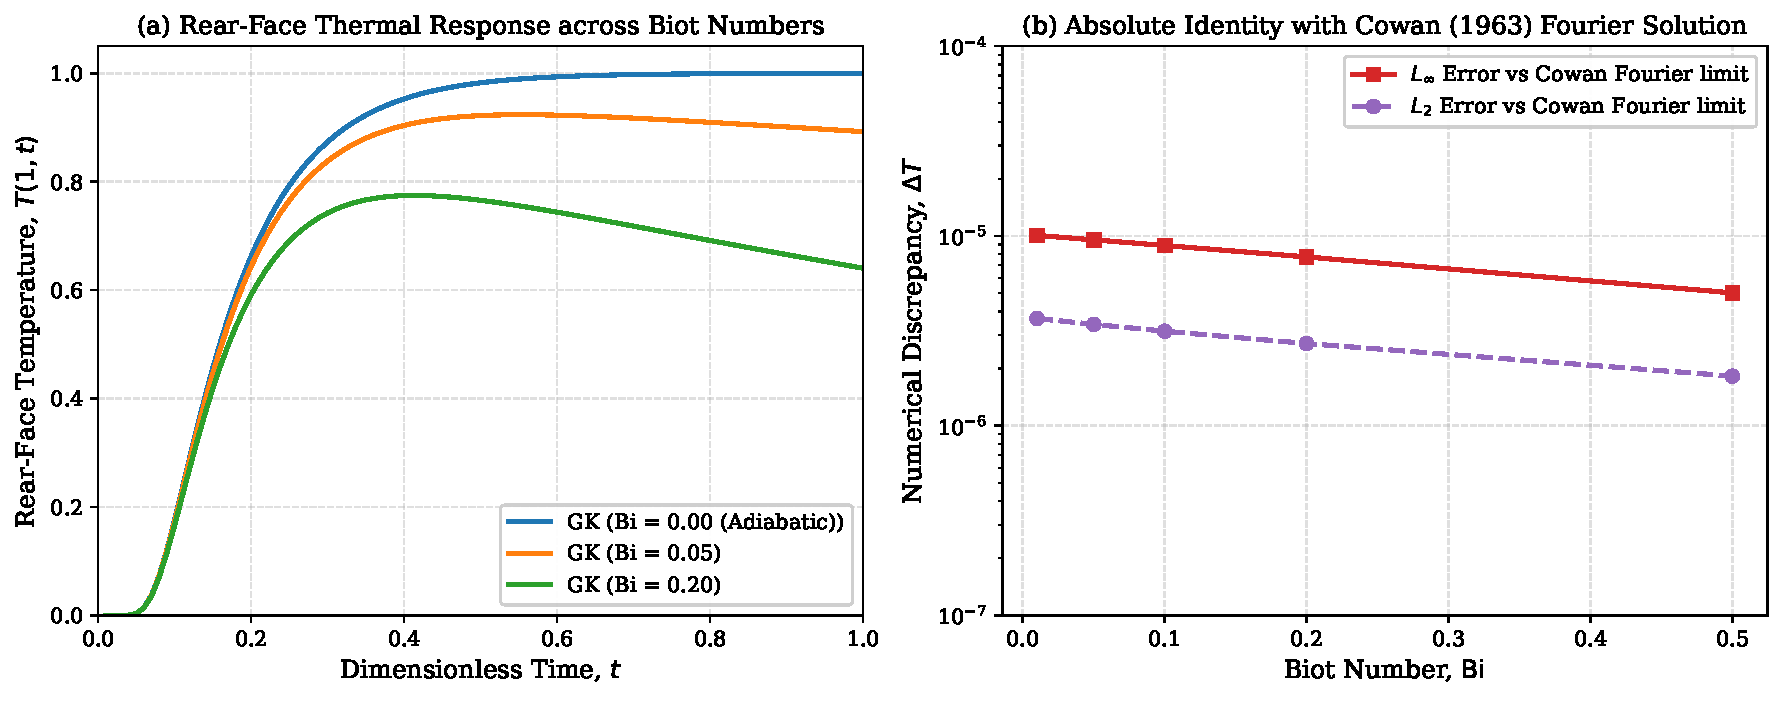
\includegraphics[width=\textwidth]{figures/fig1_heatloss_temperature_response.pdf}
\caption{(a) Rear-face temperature histories $\theta(1, t)$ for varying Biot numbers $Bi \in \{0.00, 0.05, 0.20\}$ demonstrating peak suppression and cooling tails. (b) Numerical discrepancy between GK ($B=1$) and Cowan Fourier heat conduction solutions, confirming mathematical equivalence.}
\label{fig:fig1}
\end{figure}

\subsection{Persistent Sensitivity Collinearity}

Figure~\ref{fig:fig2}(a) illustrates the time-resolved sensitivity profiles $\bm{J}_{\tau_q}(t) = \partial \theta / \partial \tau_q$ and $-\alpha_0 \bm{J}_{\kappa^2}(t) = -\alpha_0 \partial \theta / \partial \kappa^2$ for both adiabatic ($Bi = 0$) and convective ($Bi = 0.2$) cases. In both regimes, the two curves fall precisely onto each other with zero visible separation at any time instant. 

Conversely, Figure~\ref{fig:fig2}(b) plots the sensitivity with respect to the Biot number, $\bm{J}_{Bi}(t) = \partial \theta / \partial Bi$. Unlike the non-Fourier parameters, $\bm{J}_{Bi}$ exhibits a distinctly different temporal profile characterized by a sustained negative tail extending well into the cooling phase.

\begin{figure}[htbp]
\centering
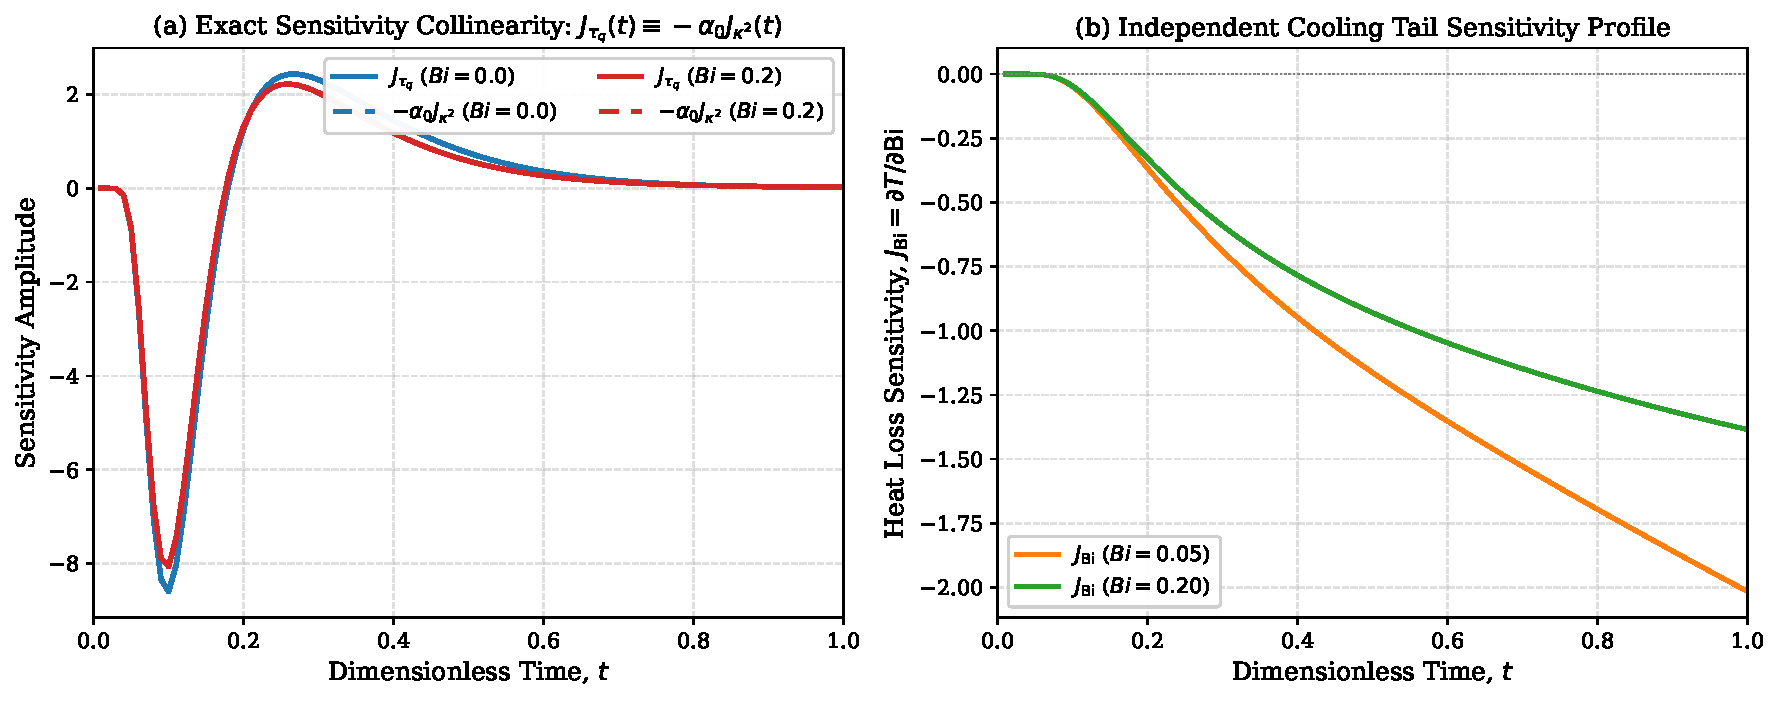
\includegraphics[width=\textwidth]{figures/fig2_sensitivity_profiles_collinearity.pdf}
\caption{(a) Front- and rear-face sensitivity profiles $\bm{J}_{\tau_q}(t)$ and $-\alpha_0 \bm{J}_{\kappa^2}(t)$ for adiabatic and convective cooling, displaying exact point-by-point overlay. (b) Independent sensitivity profile $\bm{J}_{Bi}(t) = \partial \theta / \partial Bi$ associated with the cooling tail.}
\label{fig:fig2}
\end{figure}

\subsection{Invariance Metrics Across Biot Numbers}

To rigorously quantify the robustness of this degeneracy, Table~\ref{tab:sweep} reports the collinearity correlation coefficient $\rho$, defect $|1+\rho|$, normalized residual norm $R_J = \|\bm{J}_{\tau_q} + \alpha_0 \bm{J}_{\kappa^2}\| / \|\bm{J}_{\tau_q}\|$, and condition numbers across $Bi \in [0.000, 0.500]$.

Across all Biot numbers, $\rho = -1.0000000000$, with the defect $|1+\rho|$ bounded by machine epsilon ($2.22 \times 10^{-16}$). The residual norm remains flat at $R_J \approx (5.37 - 8.11) \times 10^{-9}$, which represents the truncation error of the central finite-difference sensitivity approximation. Consequently, as shown in Figure~\ref{fig:fig3}, the condition number of the $2 \times 2$ Fisher matrix remains pinned at the numerical singularity floor $\sim 10^{17}$.

\begin{table}[htbp]
\centering
\caption{Systematic parameter sweep across Biot numbers at Fourier resonance ($B = 1.0$): Collinearity metrics, singular spectrum, and condition numbers.}
\label{tab:sweep}
\resizebox{\textwidth}{!}{
\begin{tabular}{ccccccccc}
\toprule
$Bi$ & Correlation $\rho$ & $|1+\rho|$ & Residual $R_J$ & $\sigma_1$ & $\sigma_2$ & $\sigma_3$ & $\sigma_1/\sigma_2$ & $\operatorname{cond}(F_{3\times 3})$ \\
\midrule
0.000 & -1.0000000000 & $1.11 \times 10^{-16}$ & $5.37 \times 10^{-9}$ & 31.82 & 13.57 & $7.37 \times 10^{-8}$ & 2.34 & $1.86 \times 10^{17}$ \\
0.001 & -1.0000000000 & $1.11 \times 10^{-16}$ & $5.37 \times 10^{-9}$ & 31.81 & 13.55 & $7.35 \times 10^{-8}$ & 2.35 & $1.87 \times 10^{17}$ \\
0.005 & -1.0000000000 & $0.00 \times 10^{00}$ & $5.38 \times 10^{-9}$ & 31.75 & 13.44 & $7.36 \times 10^{-8}$ & 2.36 & $1.86 \times 10^{17}$ \\
0.010 & -1.0000000000 & $2.22 \times 10^{-16}$ & $5.39 \times 10^{-9}$ & 31.68 & 13.30 & $7.36 \times 10^{-8}$ & 2.38 & $1.85 \times 10^{17}$ \\
0.050 & -1.0000000000 & $0.00 \times 10^{00}$ & $5.41 \times 10^{-9}$ & 31.13 & 12.27 & $7.25 \times 10^{-8}$ & 2.54 & $1.84 \times 10^{17}$ \\
0.100 & -1.0000000000 & $1.11 \times 10^{-16}$ & $5.48 \times 10^{-9}$ & 30.47 & 11.11 & $7.16 \times 10^{-8}$ & 2.74 & $1.81 \times 10^{17}$ \\
0.200 & -1.0000000000 & $1.11 \times 10^{-16}$ & $8.11 \times 10^{-9}$ & 29.27 & 9.15 & $1.10 \times 10^{-7}$ & 3.20 & $7.05 \times 10^{16}$ \\
0.500 & -1.0000000000 & $1.11 \times 10^{-16}$ & $5.81 \times 10^{-9}$ & 26.25 & 5.35 & $6.50 \times 10^{-8}$ & 4.90 & $1.63 \times 10^{17}$ \\
\bottomrule
\end{tabular}
}
\end{table}

\begin{figure}[htbp]
\centering
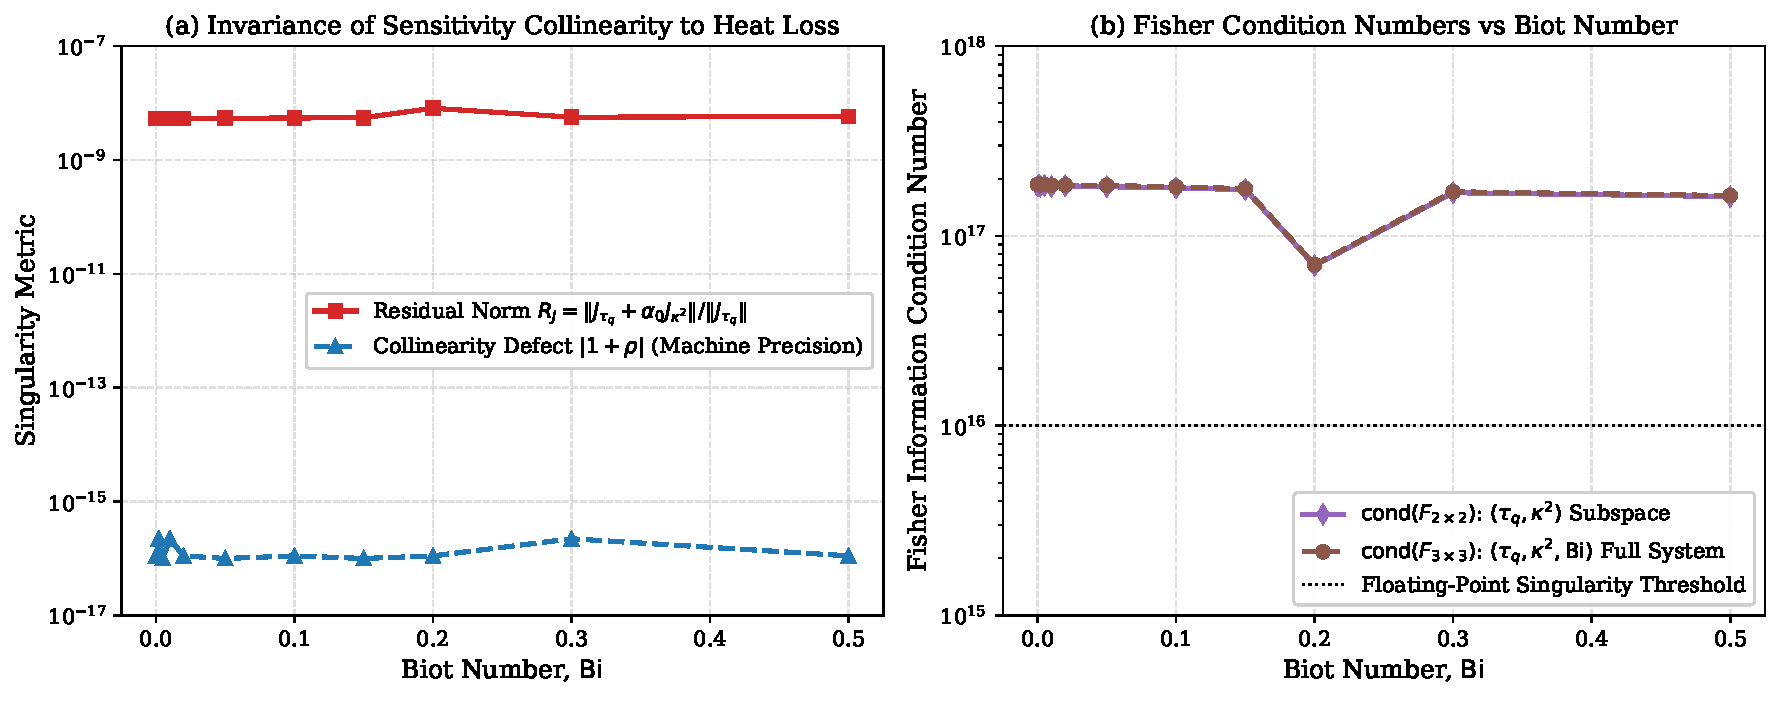
\includegraphics[width=\textwidth]{figures/fig3_invariance_metrics_vs_biot.pdf}
\caption{(a) Collinearity metrics $\log_{10}(R_J)$ and $\log_{10}(|1+\rho|)$ as functions of Biot number, demonstrating exact horizontal invariance. (b) Condition numbers $\operatorname{cond}(F_{2\times 2})$ and $\operatorname{cond}(F_{3\times 3})$ pinned at the numerical singularity floor $\sim 10^{17}$.}
\label{fig:fig3}
\end{figure}

\subsection{Singular Spectrum and Resonance Canyon}

In the full 3-parameter system $(\tau_q, \kappa^2, Bi)$, singular value decomposition reveals the underlying structural geometry:
\begin{enumerate}
    \item The leading singular value $\sigma_1 \in [26.2, 31.8]$ corresponds to the principal thermal diffusion mode.
    \item The second singular value $\sigma_2 \in [5.35, 13.57]$ corresponds directly to the convective cooling tail. The condition ratio of this observable subspace is $\sigma_1 / \sigma_2 \in [2.34, 4.90]$, indicating that the Biot number $Bi$ can be estimated with high statistical precision within this measurement framework.
    \item The third singular value $\sigma_3 \sim 10^{-8}$ corresponds strictly to the null vector $\bm{v}_{\mathrm{null}} = (1, \alpha_0, 0)^\top$, matching the theoretical eigenvector to $1.000000$ (6 decimal places). 
\end{enumerate}
As illustrated in Figure~\ref{fig:fig4}(a), boundary heat loss populates an entirely orthogonal dimension in parameter space without projecting onto the null vector. 

Finally, Figure~\ref{fig:fig4}(b) displays the condition number $\operatorname{cond}(F_{2\times 2})$ as a function of the resonance ratio $B \in [0.2, 2.0]$. Away from resonance (e.g., $B = 0.5$ or $B = 1.5$), the condition number drops sharply to moderate values ($\sim 10^2$), where heat loss causes minor quantitative shifts. However, at $B = 1.0$, an ultra-sharp singularity canyon occurs where $\operatorname{cond}(F)$ spikes to $10^{17}$, regardless of whether $Bi = 0$, $Bi = 0.05$, or $Bi = 0.20$.

\begin{figure}[htbp]
\centering
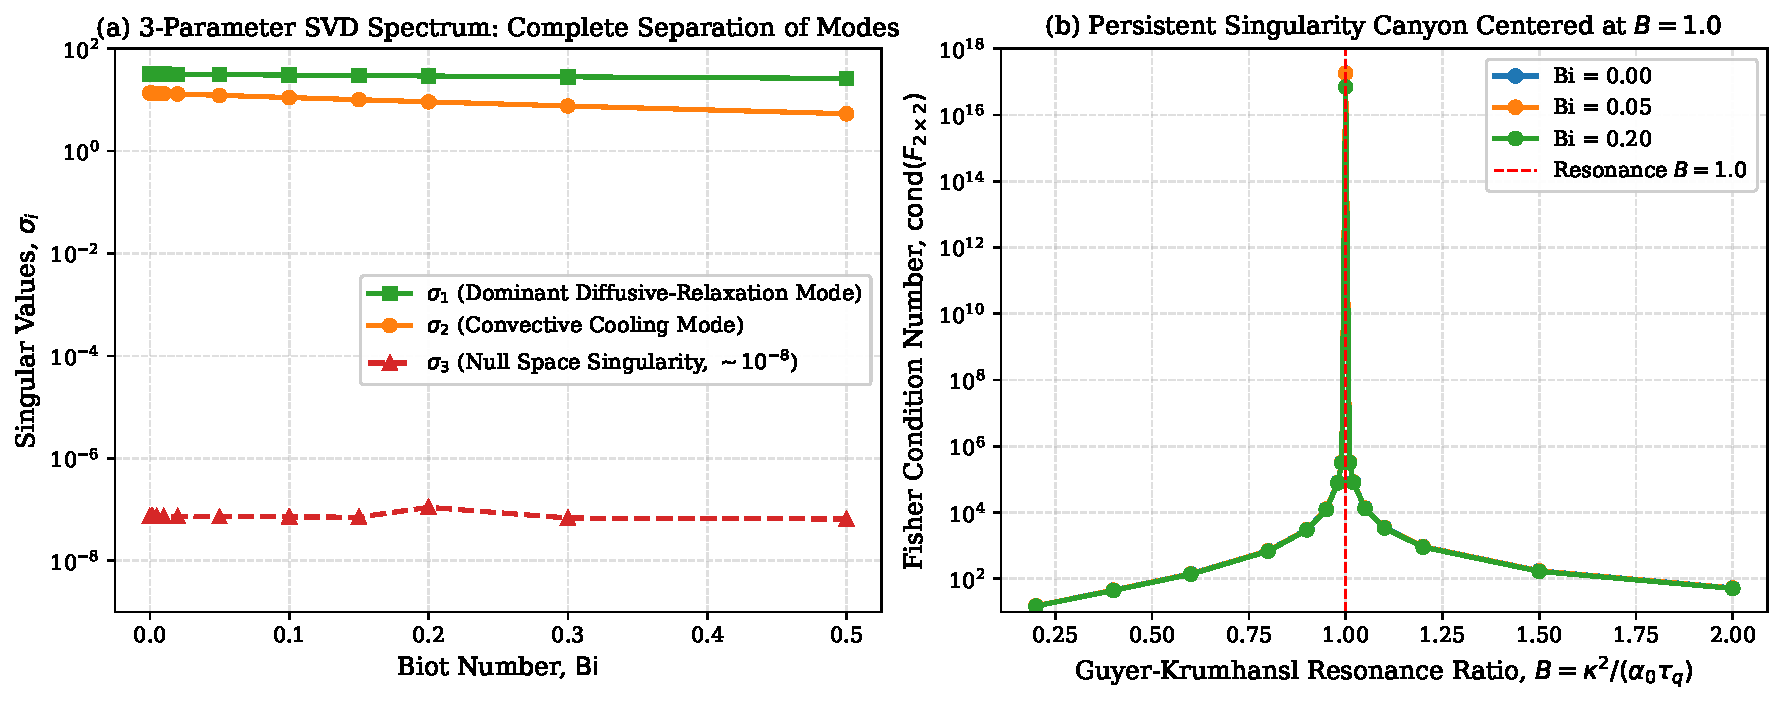
\includegraphics[width=\textwidth]{figures/fig4_singular_spectrum_and_canyon.pdf}
\caption{(a) SVD spectrum $(\sigma_1, \sigma_2, \sigma_3)$ across Biot numbers, showing clean isolation of the null singularity $\sigma_3 \sim 10^{-8}$. (b) The Fourier-resonance singularity canyon centered at $B = 1.0$, demonstrating persistent collinearity across all Biot numbers.}
\label{fig:fig4}
\end{figure}

\subsection{Asymmetric Boundary Losses and Spatial Invariance}

To ensure that Theorem~1 is not an artifact of equal front and rear heat-transfer coefficients, independent simulations were conducted for highly asymmetric pairs: $(Bi_0, Bi_L) \in \{(0.01, 0.10), (0.05, 0.20), (0.10, 0.50)\}$. In all cases, the analytical difference $|\theta_{\mathrm{GK}}(x, t)|_{B=1} - \theta_{\mathrm{Fourier}}(x, t)|$ evaluated via continuous de Hoog Laplace inversion is identically $0.00 \times 10^0$ across all time and spatial locations. Furthermore, probing interior spatial points ($x = 0.25, 0.50, 0.75$) and the front surface ($x = 0.0$) confirms field-level identity with zero residual error. Alternative thermal excitations, such as square heating pulses, yield the exact same collapse, verifying that the invariance is an intrinsic structural property of the linear Robin-boundary Guyer--Krumhansl system.

\subsection{Physical Contrast with Bulk Constitutive Nonlinearity}

It is instructive to contrast the present findings with recent investigations on bulk constitutive nonlinearities in non-Fourier transport. In companion studies on high-fluence laser flash testing, temperature-dependent thermal conductivity $\lambda(T) = \lambda_0(1 + \beta_T \theta)$ produces a non-uniform local diffusivity $\alpha(x, t) = \alpha_0(1 + \beta_T \theta(x, t))$. This internal temperature gradient destroys the uniform condition $\kappa^2 / (\alpha(x, t) \tau_q) = 1$ throughout the specimen, regularizing the Fisher condition number from $10^{17}$ to $7.3 \times 10^3$. 

This comparison illuminates a fundamental physical principle: linear boundary mechanisms (such as surface Robin cooling) preserve the spatial uniformity of the bulk propagation factor and dynamic impedance, thereby leaving the Fourier-resonance degeneracy strictly intact. Regularization of the $(\tau_q, \kappa^2)$ sensitivity singularity requires modifying the bulk transport state internally.

---

\section{Experimental Implications and Regularization Pathways}

The mathematical invariance established herein has immediate, practical consequences for laser flash thermal characterization:

\begin{enumerate}
    \item \textbf{Insufficiency of Standard Heat-Loss Corrections:} In experimental laser flash analysis, experimentalists routinely fit cooling tails to extract heat-loss coefficients (Cowan or Cape--Lehman methods) under the assumption that the extended transient signal provides sufficient information to identify non-Fourier parameters. Theorem~1 proves that for materials operating near Fourier resonance ($B \approx 1$), standard heat-loss corrections cannot resolve the indeterminacy between $\tau_q$ and $\kappa^2$. Any combination on the line $\kappa^2 = \alpha_0 \tau_q$ fits the rear-face temperature rise and cooling tail with identical fidelity.
    \item \textbf{Sample Thickness Tuning ($L$):} For homogeneous bulk materials with constant physical properties, the resonance ratio $B \equiv \frac{\kappa^2}{\alpha_0 \tau_q}$ is scale-invariant and does not change with specimen thickness $L$. However, reducing specimen thickness shortens the diffusion timescale $t_{\mathrm{diff}} = L^2 / \alpha_0$, amplifying the non-dimensional relaxation parameter $\hat{\tau}_q = \alpha_0 \tau_q / L^2$. In practical testing where a material is slightly off-resonance ($B \approx 1 \pm \delta$), reducing $L$ significantly enhances sensitivity amplitudes, moving the estimation problem out of the ill-conditioned canyon. Furthermore, in nanolayers where boundary scattering induces size-dependent mean free paths ($\kappa = \kappa(L)$), thickness tuning physically shifts $B$ away from unity.
    \item \textbf{Multi-Thickness Joint Inversion:} At exact mathematical resonance ($B \equiv 1$), specimens of all thicknesses collapse identically to their respective Fourier diffusion curves; hence joint inversion across multiple thicknesses cannot lift the exact null space without additional physical mechanisms. However, in practical testing where $B \ne 1$, simultaneously fitting transient responses across multiple thickness samples provides powerful regularization that constrains the objective function and suppresses experimental noise.
    \item \textbf{Nonlinear Excitation Regimes:} Operating at higher laser pulse fluences to induce mild temperature-dependent conductivity provides a verified physical pathway to break the internal resonance condition without altering specimen geometry.
\end{enumerate}

---

\section{Conclusions}

In this study, we investigated the effect of convective and radiative boundary heat loss on the Guyer--Krumhansl parameter identifiability singularity at Fourier resonance ($B = 1$). Through analytical derivation in the Laplace domain and high-order numerical simulations across three decades of Biot numbers ($Bi \in [0.001, 0.5]$), we established the following conclusions:
\begin{enumerate}
    \item \textbf{Invariance Theorem:} At $B \equiv \kappa^2 / (\alpha_0 \tau_q) = 1$, the Guyer--Krumhansl temperature field collapses identically to the classical Fourier heat conduction solution with the corresponding Robin boundary conditions. The dynamic surface thermal conductivity operator collapses simultaneously: $\lambda_{\mathrm{eff}}(s) \equiv \lambda_0$.
    \item \textbf{Persistence of Sensitivity Singularity:} Boundary heat loss does not break the local sensitivity collinearity $\partial T / \partial \tau_q = -\alpha_0 \partial T / \partial \kappa^2$. Across all tested Biot numbers, the correlation coefficient remains $\rho \equiv -1.0000000000$, and the condition number of the Fisher information matrix remains at the numerical singularity floor ($\sim 10^{17}$).
    \item \textbf{Subspace Separation:} In a simultaneous 3-parameter estimation framework $(\tau_q, \kappa^2, Bi)$, the cooling parameter $Bi$ is cleanly identifiable from the cooling tail with an observable condition ratio $\sigma_1 / \sigma_2 \in [2.34, 4.90]$. However, the null space $(1, \alpha_0, 0)^\top$ ($\sigma_3 \sim 10^{-8}$) remains strictly unregularized.
    \item \textbf{Asymmetric and Spatial Robustness:} The invariance theorem holds for arbitrary asymmetric heat-loss configurations ($Bi_0 \ne Bi_L$), full-field interior spatial locations, and alternative pulse profiles.
    \item \textbf{Experimental Significance:} Standard laser flash heat-loss correction procedures cannot resolve the structural identifiability degeneracy in materials near Fourier resonance. Experimentalists must instead employ strategies that perturb the bulk transport condition, such as operating in thickness regimes with size-dependent nonlocality, conducting multi-thickness joint inversions away from resonance, or utilizing high-fluence nonlinear excitation.
\end{enumerate}

\section*{Declaration of Competing Interest}
The author declares that he has no known competing financial interests or personal relationships that could have appeared to influence the work reported in this paper.

\section*{Data Availability}
All raw simulation data, calculation scripts, figure generators, and reproducibility runners are fully open-source and preserved in the repository package.

\bibliographystyle{elsarticle-num}
\bibliography{references}

\end{document}
